% Created by tikzDevice version 0.12.3 on 2020-05-01 12:40:10
% !TEX encoding = UTF-8 Unicode
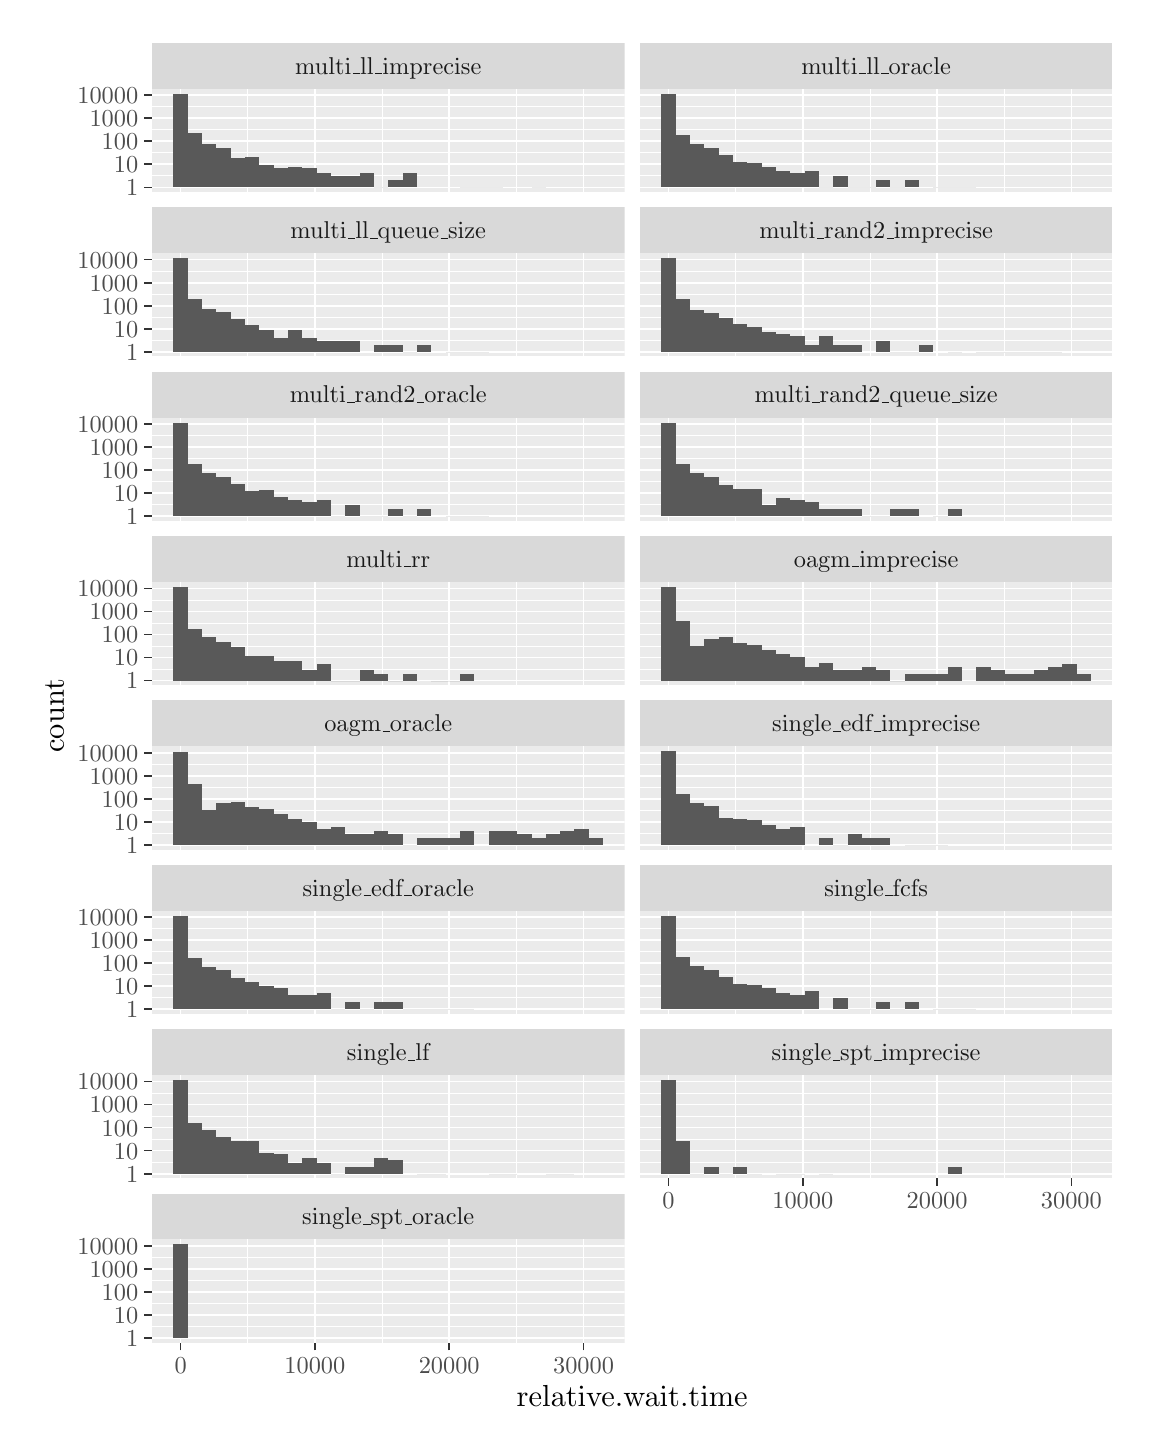
\begin{tikzpicture}[x=1pt,y=1pt]
\definecolor{fillColor}{RGB}{255,255,255}
\path[use as bounding box,fill=fillColor,fill opacity=0.00] (0,0) rectangle (397.48,505.89);
\begin{scope}
\path[clip] (  0.00,  0.00) rectangle (397.48,505.89);
\definecolor{drawColor}{RGB}{255,255,255}
\definecolor{fillColor}{RGB}{255,255,255}

\path[draw=drawColor,line width= 0.6pt,line join=round,line cap=round,fill=fillColor] (  0.00,  0.00) rectangle (397.48,505.89);
\end{scope}
\begin{scope}
\path[clip] ( 44.91,446.49) rectangle (215.70,483.82);
\definecolor{fillColor}{gray}{0.92}

\path[fill=fillColor] ( 44.91,446.49) rectangle (215.70,483.82);
\definecolor{drawColor}{RGB}{255,255,255}

\path[draw=drawColor,line width= 0.3pt,line join=round] ( 44.91,452.35) --
	(215.70,452.35);

\path[draw=drawColor,line width= 0.3pt,line join=round] ( 44.91,460.67) --
	(215.70,460.67);

\path[draw=drawColor,line width= 0.3pt,line join=round] ( 44.91,468.98) --
	(215.70,468.98);

\path[draw=drawColor,line width= 0.3pt,line join=round] ( 44.91,477.30) --
	(215.70,477.30);

\path[draw=drawColor,line width= 0.3pt,line join=round] ( 79.53,446.49) --
	( 79.53,483.82);

\path[draw=drawColor,line width= 0.3pt,line join=round] (128.06,446.49) --
	(128.06,483.82);

\path[draw=drawColor,line width= 0.3pt,line join=round] (176.60,446.49) --
	(176.60,483.82);

\path[draw=drawColor,line width= 0.6pt,line join=round] ( 44.91,448.19) --
	(215.70,448.19);

\path[draw=drawColor,line width= 0.6pt,line join=round] ( 44.91,456.51) --
	(215.70,456.51);

\path[draw=drawColor,line width= 0.6pt,line join=round] ( 44.91,464.82) --
	(215.70,464.82);

\path[draw=drawColor,line width= 0.6pt,line join=round] ( 44.91,473.14) --
	(215.70,473.14);

\path[draw=drawColor,line width= 0.6pt,line join=round] ( 44.91,481.46) --
	(215.70,481.46);

\path[draw=drawColor,line width= 0.6pt,line join=round] ( 55.26,446.49) --
	( 55.26,483.82);

\path[draw=drawColor,line width= 0.6pt,line join=round] (103.79,446.49) --
	(103.79,483.82);

\path[draw=drawColor,line width= 0.6pt,line join=round] (152.33,446.49) --
	(152.33,483.82);

\path[draw=drawColor,line width= 0.6pt,line join=round] (200.86,446.49) --
	(200.86,483.82);
\definecolor{fillColor}{gray}{0.35}

\path[fill=fillColor] ( 52.67,448.19) rectangle ( 57.85,481.99);

\path[fill=fillColor] ( 57.85,448.19) rectangle ( 63.02,467.71);

\path[fill=fillColor] ( 63.02,448.19) rectangle ( 68.20,463.79);

\path[fill=fillColor] ( 68.20,448.19) rectangle ( 73.37,462.39);

\path[fill=fillColor] ( 73.37,448.19) rectangle ( 78.55,458.63);

\path[fill=fillColor] ( 78.55,448.19) rectangle ( 83.72,459.01);

\path[fill=fillColor] ( 83.72,448.19) rectangle ( 88.90,456.12);

\path[fill=fillColor] ( 88.90,448.19) rectangle ( 94.08,455.22);

\path[fill=fillColor] ( 94.08,448.19) rectangle ( 99.25,455.70);

\path[fill=fillColor] ( 99.25,448.19) rectangle (104.43,455.22);

\path[fill=fillColor] (104.43,448.19) rectangle (109.60,453.19);

\path[fill=fillColor] (109.60,448.19) rectangle (114.78,452.16);

\path[fill=fillColor] (114.78,448.19) rectangle (119.95,452.16);

\path[fill=fillColor] (119.95,448.19) rectangle (125.13,453.19);

\path[fill=fillColor] (125.13,448.19) rectangle (130.30,448.19);

\path[fill=fillColor] (130.30,448.19) rectangle (135.48,450.69);

\path[fill=fillColor] (135.48,448.19) rectangle (140.65,453.19);

\path[fill=fillColor] (156.18,448.19) rectangle (161.36,448.19);

\path[fill=fillColor] (161.36,448.19) rectangle (166.53,448.19);

\path[fill=fillColor] (166.53,448.19) rectangle (171.71,448.19);

\path[fill=fillColor] (182.06,448.19) rectangle (187.23,448.19);
\end{scope}
\begin{scope}
\path[clip] ( 44.91,387.09) rectangle (215.70,424.42);
\definecolor{fillColor}{gray}{0.92}

\path[fill=fillColor] ( 44.91,387.09) rectangle (215.70,424.42);
\definecolor{drawColor}{RGB}{255,255,255}

\path[draw=drawColor,line width= 0.3pt,line join=round] ( 44.91,392.95) --
	(215.70,392.95);

\path[draw=drawColor,line width= 0.3pt,line join=round] ( 44.91,401.26) --
	(215.70,401.26);

\path[draw=drawColor,line width= 0.3pt,line join=round] ( 44.91,409.58) --
	(215.70,409.58);

\path[draw=drawColor,line width= 0.3pt,line join=round] ( 44.91,417.90) --
	(215.70,417.90);

\path[draw=drawColor,line width= 0.3pt,line join=round] ( 79.53,387.09) --
	( 79.53,424.42);

\path[draw=drawColor,line width= 0.3pt,line join=round] (128.06,387.09) --
	(128.06,424.42);

\path[draw=drawColor,line width= 0.3pt,line join=round] (176.60,387.09) --
	(176.60,424.42);

\path[draw=drawColor,line width= 0.6pt,line join=round] ( 44.91,388.79) --
	(215.70,388.79);

\path[draw=drawColor,line width= 0.6pt,line join=round] ( 44.91,397.10) --
	(215.70,397.10);

\path[draw=drawColor,line width= 0.6pt,line join=round] ( 44.91,405.42) --
	(215.70,405.42);

\path[draw=drawColor,line width= 0.6pt,line join=round] ( 44.91,413.74) --
	(215.70,413.74);

\path[draw=drawColor,line width= 0.6pt,line join=round] ( 44.91,422.06) --
	(215.70,422.06);

\path[draw=drawColor,line width= 0.6pt,line join=round] ( 55.26,387.09) --
	( 55.26,424.42);

\path[draw=drawColor,line width= 0.6pt,line join=round] (103.79,387.09) --
	(103.79,424.42);

\path[draw=drawColor,line width= 0.6pt,line join=round] (152.33,387.09) --
	(152.33,424.42);

\path[draw=drawColor,line width= 0.6pt,line join=round] (200.86,387.09) --
	(200.86,424.42);
\definecolor{fillColor}{gray}{0.35}

\path[fill=fillColor] ( 52.67,388.79) rectangle ( 57.85,422.60);

\path[fill=fillColor] ( 57.85,388.79) rectangle ( 63.02,407.67);

\path[fill=fillColor] ( 63.02,388.79) rectangle ( 68.20,404.34);

\path[fill=fillColor] ( 68.20,388.79) rectangle ( 73.37,403.06);

\path[fill=fillColor] ( 73.37,388.79) rectangle ( 78.55,400.56);

\path[fill=fillColor] ( 78.55,388.79) rectangle ( 83.72,398.57);

\path[fill=fillColor] ( 83.72,388.79) rectangle ( 88.90,396.72);

\path[fill=fillColor] ( 88.90,388.79) rectangle ( 94.08,393.79);

\path[fill=fillColor] ( 94.08,388.79) rectangle ( 99.25,396.72);

\path[fill=fillColor] ( 99.25,388.79) rectangle (104.43,393.79);

\path[fill=fillColor] (104.43,388.79) rectangle (109.60,392.75);

\path[fill=fillColor] (109.60,388.79) rectangle (114.78,392.75);

\path[fill=fillColor] (114.78,388.79) rectangle (119.95,392.75);

\path[fill=fillColor] (125.13,388.79) rectangle (130.30,391.29);

\path[fill=fillColor] (130.30,388.79) rectangle (135.48,391.29);

\path[fill=fillColor] (135.48,388.79) rectangle (140.65,388.79);

\path[fill=fillColor] (140.65,388.79) rectangle (145.83,391.29);

\path[fill=fillColor] (151.00,388.79) rectangle (156.18,388.79);

\path[fill=fillColor] (156.18,388.79) rectangle (161.36,388.79);

\path[fill=fillColor] (161.36,388.79) rectangle (166.53,388.79);
\end{scope}
\begin{scope}
\path[clip] ( 44.91,327.69) rectangle (215.70,365.02);
\definecolor{fillColor}{gray}{0.92}

\path[fill=fillColor] ( 44.91,327.69) rectangle (215.70,365.02);
\definecolor{drawColor}{RGB}{255,255,255}

\path[draw=drawColor,line width= 0.3pt,line join=round] ( 44.91,333.54) --
	(215.70,333.54);

\path[draw=drawColor,line width= 0.3pt,line join=round] ( 44.91,341.86) --
	(215.70,341.86);

\path[draw=drawColor,line width= 0.3pt,line join=round] ( 44.91,350.18) --
	(215.70,350.18);

\path[draw=drawColor,line width= 0.3pt,line join=round] ( 44.91,358.50) --
	(215.70,358.50);

\path[draw=drawColor,line width= 0.3pt,line join=round] ( 79.53,327.69) --
	( 79.53,365.02);

\path[draw=drawColor,line width= 0.3pt,line join=round] (128.06,327.69) --
	(128.06,365.02);

\path[draw=drawColor,line width= 0.3pt,line join=round] (176.60,327.69) --
	(176.60,365.02);

\path[draw=drawColor,line width= 0.6pt,line join=round] ( 44.91,329.39) --
	(215.70,329.39);

\path[draw=drawColor,line width= 0.6pt,line join=round] ( 44.91,337.70) --
	(215.70,337.70);

\path[draw=drawColor,line width= 0.6pt,line join=round] ( 44.91,346.02) --
	(215.70,346.02);

\path[draw=drawColor,line width= 0.6pt,line join=round] ( 44.91,354.34) --
	(215.70,354.34);

\path[draw=drawColor,line width= 0.6pt,line join=round] ( 44.91,362.66) --
	(215.70,362.66);

\path[draw=drawColor,line width= 0.6pt,line join=round] ( 55.26,327.69) --
	( 55.26,365.02);

\path[draw=drawColor,line width= 0.6pt,line join=round] (103.79,327.69) --
	(103.79,365.02);

\path[draw=drawColor,line width= 0.6pt,line join=round] (152.33,327.69) --
	(152.33,365.02);

\path[draw=drawColor,line width= 0.6pt,line join=round] (200.86,327.69) --
	(200.86,365.02);
\definecolor{fillColor}{gray}{0.35}

\path[fill=fillColor] ( 52.67,329.39) rectangle ( 57.85,363.20);

\path[fill=fillColor] ( 57.85,329.39) rectangle ( 63.02,348.09);

\path[fill=fillColor] ( 63.02,329.39) rectangle ( 68.20,345.13);

\path[fill=fillColor] ( 68.20,329.39) rectangle ( 73.37,343.59);

\path[fill=fillColor] ( 73.37,329.39) rectangle ( 78.55,341.16);

\path[fill=fillColor] ( 78.55,329.39) rectangle ( 83.72,338.36);

\path[fill=fillColor] ( 83.72,329.39) rectangle ( 88.90,338.65);

\path[fill=fillColor] ( 88.90,329.39) rectangle ( 94.08,336.42);

\path[fill=fillColor] ( 94.08,329.39) rectangle ( 99.25,335.20);

\path[fill=fillColor] ( 99.25,329.39) rectangle (104.43,334.39);

\path[fill=fillColor] (104.43,329.39) rectangle (109.60,335.20);

\path[fill=fillColor] (109.60,329.39) rectangle (114.78,329.39);

\path[fill=fillColor] (114.78,329.39) rectangle (119.95,333.35);

\path[fill=fillColor] (119.95,329.39) rectangle (125.13,329.39);

\path[fill=fillColor] (125.13,329.39) rectangle (130.30,329.39);

\path[fill=fillColor] (130.30,329.39) rectangle (135.48,331.89);

\path[fill=fillColor] (135.48,329.39) rectangle (140.65,329.39);

\path[fill=fillColor] (140.65,329.39) rectangle (145.83,331.89);

\path[fill=fillColor] (151.00,329.39) rectangle (156.18,329.39);

\path[fill=fillColor] (156.18,329.39) rectangle (161.36,329.39);

\path[fill=fillColor] (161.36,329.39) rectangle (166.53,329.39);
\end{scope}
\begin{scope}
\path[clip] ( 44.91,268.29) rectangle (215.70,305.62);
\definecolor{fillColor}{gray}{0.92}

\path[fill=fillColor] ( 44.91,268.29) rectangle (215.70,305.62);
\definecolor{drawColor}{RGB}{255,255,255}

\path[draw=drawColor,line width= 0.3pt,line join=round] ( 44.91,274.14) --
	(215.70,274.14);

\path[draw=drawColor,line width= 0.3pt,line join=round] ( 44.91,282.46) --
	(215.70,282.46);

\path[draw=drawColor,line width= 0.3pt,line join=round] ( 44.91,290.78) --
	(215.70,290.78);

\path[draw=drawColor,line width= 0.3pt,line join=round] ( 44.91,299.10) --
	(215.70,299.10);

\path[draw=drawColor,line width= 0.3pt,line join=round] ( 79.53,268.29) --
	( 79.53,305.62);

\path[draw=drawColor,line width= 0.3pt,line join=round] (128.06,268.29) --
	(128.06,305.62);

\path[draw=drawColor,line width= 0.3pt,line join=round] (176.60,268.29) --
	(176.60,305.62);

\path[draw=drawColor,line width= 0.6pt,line join=round] ( 44.91,269.98) --
	(215.70,269.98);

\path[draw=drawColor,line width= 0.6pt,line join=round] ( 44.91,278.30) --
	(215.70,278.30);

\path[draw=drawColor,line width= 0.6pt,line join=round] ( 44.91,286.62) --
	(215.70,286.62);

\path[draw=drawColor,line width= 0.6pt,line join=round] ( 44.91,294.94) --
	(215.70,294.94);

\path[draw=drawColor,line width= 0.6pt,line join=round] ( 44.91,303.26) --
	(215.70,303.26);

\path[draw=drawColor,line width= 0.6pt,line join=round] ( 55.26,268.29) --
	( 55.26,305.62);

\path[draw=drawColor,line width= 0.6pt,line join=round] (103.79,268.29) --
	(103.79,305.62);

\path[draw=drawColor,line width= 0.6pt,line join=round] (152.33,268.29) --
	(152.33,305.62);

\path[draw=drawColor,line width= 0.6pt,line join=round] (200.86,268.29) --
	(200.86,305.62);
\definecolor{fillColor}{gray}{0.35}

\path[fill=fillColor] ( 52.67,269.98) rectangle ( 57.85,303.80);

\path[fill=fillColor] ( 57.85,269.98) rectangle ( 63.02,288.69);

\path[fill=fillColor] ( 63.02,269.98) rectangle ( 68.20,285.73);

\path[fill=fillColor] ( 68.20,269.98) rectangle ( 73.37,284.05);

\path[fill=fillColor] ( 73.37,269.98) rectangle ( 78.55,282.02);

\path[fill=fillColor] ( 78.55,269.98) rectangle ( 83.72,278.96);

\path[fill=fillColor] ( 83.72,269.98) rectangle ( 88.90,278.96);

\path[fill=fillColor] ( 88.90,269.98) rectangle ( 94.08,277.02);

\path[fill=fillColor] ( 94.08,269.98) rectangle ( 99.25,277.02);

\path[fill=fillColor] ( 99.25,269.98) rectangle (104.43,273.95);

\path[fill=fillColor] (104.43,269.98) rectangle (109.60,275.80);

\path[fill=fillColor] (109.60,269.98) rectangle (114.78,269.98);

\path[fill=fillColor] (114.78,269.98) rectangle (119.95,269.98);

\path[fill=fillColor] (119.95,269.98) rectangle (125.13,273.95);

\path[fill=fillColor] (125.13,269.98) rectangle (130.30,272.49);

\path[fill=fillColor] (130.30,269.98) rectangle (135.48,269.98);

\path[fill=fillColor] (135.48,269.98) rectangle (140.65,272.49);

\path[fill=fillColor] (145.83,269.98) rectangle (151.00,269.98);

\path[fill=fillColor] (151.00,269.98) rectangle (156.18,269.98);

\path[fill=fillColor] (156.18,269.98) rectangle (161.36,272.49);
\end{scope}
\begin{scope}
\path[clip] ( 44.91,208.89) rectangle (215.70,246.22);
\definecolor{fillColor}{gray}{0.92}

\path[fill=fillColor] ( 44.91,208.89) rectangle (215.70,246.22);
\definecolor{drawColor}{RGB}{255,255,255}

\path[draw=drawColor,line width= 0.3pt,line join=round] ( 44.91,214.74) --
	(215.70,214.74);

\path[draw=drawColor,line width= 0.3pt,line join=round] ( 44.91,223.06) --
	(215.70,223.06);

\path[draw=drawColor,line width= 0.3pt,line join=round] ( 44.91,231.38) --
	(215.70,231.38);

\path[draw=drawColor,line width= 0.3pt,line join=round] ( 44.91,239.70) --
	(215.70,239.70);

\path[draw=drawColor,line width= 0.3pt,line join=round] ( 79.53,208.89) --
	( 79.53,246.22);

\path[draw=drawColor,line width= 0.3pt,line join=round] (128.06,208.89) --
	(128.06,246.22);

\path[draw=drawColor,line width= 0.3pt,line join=round] (176.60,208.89) --
	(176.60,246.22);

\path[draw=drawColor,line width= 0.6pt,line join=round] ( 44.91,210.58) --
	(215.70,210.58);

\path[draw=drawColor,line width= 0.6pt,line join=round] ( 44.91,218.90) --
	(215.70,218.90);

\path[draw=drawColor,line width= 0.6pt,line join=round] ( 44.91,227.22) --
	(215.70,227.22);

\path[draw=drawColor,line width= 0.6pt,line join=round] ( 44.91,235.54) --
	(215.70,235.54);

\path[draw=drawColor,line width= 0.6pt,line join=round] ( 44.91,243.86) --
	(215.70,243.86);

\path[draw=drawColor,line width= 0.6pt,line join=round] ( 55.26,208.89) --
	( 55.26,246.22);

\path[draw=drawColor,line width= 0.6pt,line join=round] (103.79,208.89) --
	(103.79,246.22);

\path[draw=drawColor,line width= 0.6pt,line join=round] (152.33,208.89) --
	(152.33,246.22);

\path[draw=drawColor,line width= 0.6pt,line join=round] (200.86,208.89) --
	(200.86,246.22);
\definecolor{fillColor}{gray}{0.35}

\path[fill=fillColor] ( 52.67,210.58) rectangle ( 57.85,244.27);

\path[fill=fillColor] ( 57.85,210.58) rectangle ( 63.02,232.48);

\path[fill=fillColor] ( 63.02,210.58) rectangle ( 68.20,223.22);

\path[fill=fillColor] ( 68.20,210.58) rectangle ( 73.37,225.67);

\path[fill=fillColor] ( 73.37,210.58) rectangle ( 78.55,226.23);

\path[fill=fillColor] ( 78.55,210.58) rectangle ( 83.72,224.17);

\path[fill=fillColor] ( 83.72,210.58) rectangle ( 88.90,223.53);

\path[fill=fillColor] ( 88.90,210.58) rectangle ( 94.08,221.75);

\path[fill=fillColor] ( 94.08,210.58) rectangle ( 99.25,219.85);

\path[fill=fillColor] ( 99.25,210.58) rectangle (104.43,218.90);

\path[fill=fillColor] (104.43,210.58) rectangle (109.60,216.40);

\path[fill=fillColor] (109.60,210.58) rectangle (114.78,217.06);

\path[fill=fillColor] (114.78,210.58) rectangle (119.95,214.55);

\path[fill=fillColor] (119.95,210.58) rectangle (125.13,214.55);

\path[fill=fillColor] (125.13,210.58) rectangle (130.30,215.59);

\path[fill=fillColor] (130.30,210.58) rectangle (135.48,214.55);

\path[fill=fillColor] (135.48,210.58) rectangle (140.65,210.58);

\path[fill=fillColor] (140.65,210.58) rectangle (145.83,213.09);

\path[fill=fillColor] (145.83,210.58) rectangle (151.00,213.09);

\path[fill=fillColor] (151.00,210.58) rectangle (156.18,213.09);

\path[fill=fillColor] (156.18,210.58) rectangle (161.36,215.59);

\path[fill=fillColor] (166.53,210.58) rectangle (171.71,215.59);

\path[fill=fillColor] (171.71,210.58) rectangle (176.88,215.59);

\path[fill=fillColor] (176.88,210.58) rectangle (182.06,214.55);

\path[fill=fillColor] (182.06,210.58) rectangle (187.23,213.09);

\path[fill=fillColor] (187.23,210.58) rectangle (192.41,214.55);

\path[fill=fillColor] (192.41,210.58) rectangle (197.58,215.59);

\path[fill=fillColor] (197.58,210.58) rectangle (202.76,216.40);

\path[fill=fillColor] (202.76,210.58) rectangle (207.93,213.09);
\end{scope}
\begin{scope}
\path[clip] ( 44.91,149.49) rectangle (215.70,186.82);
\definecolor{fillColor}{gray}{0.92}

\path[fill=fillColor] ( 44.91,149.49) rectangle (215.70,186.82);
\definecolor{drawColor}{RGB}{255,255,255}

\path[draw=drawColor,line width= 0.3pt,line join=round] ( 44.91,155.34) --
	(215.70,155.34);

\path[draw=drawColor,line width= 0.3pt,line join=round] ( 44.91,163.66) --
	(215.70,163.66);

\path[draw=drawColor,line width= 0.3pt,line join=round] ( 44.91,171.98) --
	(215.70,171.98);

\path[draw=drawColor,line width= 0.3pt,line join=round] ( 44.91,180.30) --
	(215.70,180.30);

\path[draw=drawColor,line width= 0.3pt,line join=round] ( 79.53,149.49) --
	( 79.53,186.82);

\path[draw=drawColor,line width= 0.3pt,line join=round] (128.06,149.49) --
	(128.06,186.82);

\path[draw=drawColor,line width= 0.3pt,line join=round] (176.60,149.49) --
	(176.60,186.82);

\path[draw=drawColor,line width= 0.6pt,line join=round] ( 44.91,151.18) --
	(215.70,151.18);

\path[draw=drawColor,line width= 0.6pt,line join=round] ( 44.91,159.50) --
	(215.70,159.50);

\path[draw=drawColor,line width= 0.6pt,line join=round] ( 44.91,167.82) --
	(215.70,167.82);

\path[draw=drawColor,line width= 0.6pt,line join=round] ( 44.91,176.14) --
	(215.70,176.14);

\path[draw=drawColor,line width= 0.6pt,line join=round] ( 44.91,184.46) --
	(215.70,184.46);

\path[draw=drawColor,line width= 0.6pt,line join=round] ( 55.26,149.49) --
	( 55.26,186.82);

\path[draw=drawColor,line width= 0.6pt,line join=round] (103.79,149.49) --
	(103.79,186.82);

\path[draw=drawColor,line width= 0.6pt,line join=round] (152.33,149.49) --
	(152.33,186.82);

\path[draw=drawColor,line width= 0.6pt,line join=round] (200.86,149.49) --
	(200.86,186.82);
\definecolor{fillColor}{gray}{0.35}

\path[fill=fillColor] ( 52.67,151.18) rectangle ( 57.85,185.01);

\path[fill=fillColor] ( 57.85,151.18) rectangle ( 63.02,169.70);

\path[fill=fillColor] ( 63.02,151.18) rectangle ( 68.20,166.32);

\path[fill=fillColor] ( 68.20,151.18) rectangle ( 73.37,165.39);

\path[fill=fillColor] ( 73.37,151.18) rectangle ( 78.55,162.35);

\path[fill=fillColor] ( 78.55,151.18) rectangle ( 83.72,160.97);

\path[fill=fillColor] ( 83.72,151.18) rectangle ( 88.90,159.50);

\path[fill=fillColor] ( 88.90,151.18) rectangle ( 94.08,158.70);

\path[fill=fillColor] ( 94.08,151.18) rectangle ( 99.25,156.19);

\path[fill=fillColor] ( 99.25,151.18) rectangle (104.43,156.19);

\path[fill=fillColor] (104.43,151.18) rectangle (109.60,157.00);

\path[fill=fillColor] (109.60,151.18) rectangle (114.78,151.18);

\path[fill=fillColor] (114.78,151.18) rectangle (119.95,153.69);

\path[fill=fillColor] (119.95,151.18) rectangle (125.13,151.18);

\path[fill=fillColor] (125.13,151.18) rectangle (130.30,153.69);

\path[fill=fillColor] (130.30,151.18) rectangle (135.48,153.69);

\path[fill=fillColor] (135.48,151.18) rectangle (140.65,151.18);

\path[fill=fillColor] (140.65,151.18) rectangle (145.83,151.18);

\path[fill=fillColor] (145.83,151.18) rectangle (151.00,151.18);

\path[fill=fillColor] (151.00,151.18) rectangle (156.18,151.18);

\path[fill=fillColor] (156.18,151.18) rectangle (161.36,151.18);
\end{scope}
\begin{scope}
\path[clip] ( 44.91, 90.09) rectangle (215.70,127.42);
\definecolor{fillColor}{gray}{0.92}

\path[fill=fillColor] ( 44.91, 90.09) rectangle (215.70,127.42);
\definecolor{drawColor}{RGB}{255,255,255}

\path[draw=drawColor,line width= 0.3pt,line join=round] ( 44.91, 95.94) --
	(215.70, 95.94);

\path[draw=drawColor,line width= 0.3pt,line join=round] ( 44.91,104.26) --
	(215.70,104.26);

\path[draw=drawColor,line width= 0.3pt,line join=round] ( 44.91,112.58) --
	(215.70,112.58);

\path[draw=drawColor,line width= 0.3pt,line join=round] ( 44.91,120.90) --
	(215.70,120.90);

\path[draw=drawColor,line width= 0.3pt,line join=round] ( 79.53, 90.09) --
	( 79.53,127.42);

\path[draw=drawColor,line width= 0.3pt,line join=round] (128.06, 90.09) --
	(128.06,127.42);

\path[draw=drawColor,line width= 0.3pt,line join=round] (176.60, 90.09) --
	(176.60,127.42);

\path[draw=drawColor,line width= 0.6pt,line join=round] ( 44.91, 91.78) --
	(215.70, 91.78);

\path[draw=drawColor,line width= 0.6pt,line join=round] ( 44.91,100.10) --
	(215.70,100.10);

\path[draw=drawColor,line width= 0.6pt,line join=round] ( 44.91,108.42) --
	(215.70,108.42);

\path[draw=drawColor,line width= 0.6pt,line join=round] ( 44.91,116.74) --
	(215.70,116.74);

\path[draw=drawColor,line width= 0.6pt,line join=round] ( 44.91,125.06) --
	(215.70,125.06);

\path[draw=drawColor,line width= 0.6pt,line join=round] ( 55.26, 90.09) --
	( 55.26,127.42);

\path[draw=drawColor,line width= 0.6pt,line join=round] (103.79, 90.09) --
	(103.79,127.42);

\path[draw=drawColor,line width= 0.6pt,line join=round] (152.33, 90.09) --
	(152.33,127.42);

\path[draw=drawColor,line width= 0.6pt,line join=round] (200.86, 90.09) --
	(200.86,127.42);
\definecolor{fillColor}{gray}{0.35}

\path[fill=fillColor] ( 52.67, 91.78) rectangle ( 57.85,125.60);

\path[fill=fillColor] ( 57.85, 91.78) rectangle ( 63.02,110.19);

\path[fill=fillColor] ( 63.02, 91.78) rectangle ( 68.20,107.52);

\path[fill=fillColor] ( 68.20, 91.78) rectangle ( 73.37,104.93);

\path[fill=fillColor] ( 73.37, 91.78) rectangle ( 78.55,103.69);

\path[fill=fillColor] ( 78.55, 91.78) rectangle ( 83.72,103.69);

\path[fill=fillColor] ( 83.72, 91.78) rectangle ( 88.90, 99.30);

\path[fill=fillColor] ( 88.90, 91.78) rectangle ( 94.08, 98.81);

\path[fill=fillColor] ( 94.08, 91.78) rectangle ( 99.25, 95.75);

\path[fill=fillColor] ( 99.25, 91.78) rectangle (104.43, 97.60);

\path[fill=fillColor] (104.43, 91.78) rectangle (109.60, 95.75);

\path[fill=fillColor] (109.60, 91.78) rectangle (114.78, 91.78);

\path[fill=fillColor] (114.78, 91.78) rectangle (119.95, 94.29);

\path[fill=fillColor] (119.95, 91.78) rectangle (125.13, 94.29);

\path[fill=fillColor] (125.13, 91.78) rectangle (130.30, 97.60);

\path[fill=fillColor] (130.30, 91.78) rectangle (135.48, 96.79);

\path[fill=fillColor] (140.65, 91.78) rectangle (145.83, 91.78);

\path[fill=fillColor] (145.83, 91.78) rectangle (151.00, 91.78);

\path[fill=fillColor] (166.53, 91.78) rectangle (171.71, 91.78);

\path[fill=fillColor] (171.71, 91.78) rectangle (176.88, 91.78);

\path[fill=fillColor] (187.23, 91.78) rectangle (192.41, 91.78);

\path[fill=fillColor] (192.41, 91.78) rectangle (197.58, 91.78);
\end{scope}
\begin{scope}
\path[clip] ( 44.91, 30.69) rectangle (215.70, 68.01);
\definecolor{fillColor}{gray}{0.92}

\path[fill=fillColor] ( 44.91, 30.69) rectangle (215.70, 68.01);
\definecolor{drawColor}{RGB}{255,255,255}

\path[draw=drawColor,line width= 0.3pt,line join=round] ( 44.91, 36.54) --
	(215.70, 36.54);

\path[draw=drawColor,line width= 0.3pt,line join=round] ( 44.91, 44.86) --
	(215.70, 44.86);

\path[draw=drawColor,line width= 0.3pt,line join=round] ( 44.91, 53.18) --
	(215.70, 53.18);

\path[draw=drawColor,line width= 0.3pt,line join=round] ( 44.91, 61.50) --
	(215.70, 61.50);

\path[draw=drawColor,line width= 0.3pt,line join=round] ( 79.53, 30.69) --
	( 79.53, 68.01);

\path[draw=drawColor,line width= 0.3pt,line join=round] (128.06, 30.69) --
	(128.06, 68.01);

\path[draw=drawColor,line width= 0.3pt,line join=round] (176.60, 30.69) --
	(176.60, 68.01);

\path[draw=drawColor,line width= 0.6pt,line join=round] ( 44.91, 32.38) --
	(215.70, 32.38);

\path[draw=drawColor,line width= 0.6pt,line join=round] ( 44.91, 40.70) --
	(215.70, 40.70);

\path[draw=drawColor,line width= 0.6pt,line join=round] ( 44.91, 49.02) --
	(215.70, 49.02);

\path[draw=drawColor,line width= 0.6pt,line join=round] ( 44.91, 57.34) --
	(215.70, 57.34);

\path[draw=drawColor,line width= 0.6pt,line join=round] ( 44.91, 65.66) --
	(215.70, 65.66);

\path[draw=drawColor,line width= 0.6pt,line join=round] ( 55.26, 30.69) --
	( 55.26, 68.01);

\path[draw=drawColor,line width= 0.6pt,line join=round] (103.79, 30.69) --
	(103.79, 68.01);

\path[draw=drawColor,line width= 0.6pt,line join=round] (152.33, 30.69) --
	(152.33, 68.01);

\path[draw=drawColor,line width= 0.6pt,line join=round] (200.86, 30.69) --
	(200.86, 68.01);
\definecolor{fillColor}{gray}{0.35}

\path[fill=fillColor] ( 52.67, 32.38) rectangle ( 57.85, 66.32);
\end{scope}
\begin{scope}
\path[clip] (221.20,446.49) rectangle (391.98,483.82);
\definecolor{fillColor}{gray}{0.92}

\path[fill=fillColor] (221.20,446.49) rectangle (391.98,483.82);
\definecolor{drawColor}{RGB}{255,255,255}

\path[draw=drawColor,line width= 0.3pt,line join=round] (221.20,452.35) --
	(391.98,452.35);

\path[draw=drawColor,line width= 0.3pt,line join=round] (221.20,460.67) --
	(391.98,460.67);

\path[draw=drawColor,line width= 0.3pt,line join=round] (221.20,468.98) --
	(391.98,468.98);

\path[draw=drawColor,line width= 0.3pt,line join=round] (221.20,477.30) --
	(391.98,477.30);

\path[draw=drawColor,line width= 0.3pt,line join=round] (255.82,446.49) --
	(255.82,483.82);

\path[draw=drawColor,line width= 0.3pt,line join=round] (304.35,446.49) --
	(304.35,483.82);

\path[draw=drawColor,line width= 0.3pt,line join=round] (352.89,446.49) --
	(352.89,483.82);

\path[draw=drawColor,line width= 0.6pt,line join=round] (221.20,448.19) --
	(391.98,448.19);

\path[draw=drawColor,line width= 0.6pt,line join=round] (221.20,456.51) --
	(391.98,456.51);

\path[draw=drawColor,line width= 0.6pt,line join=round] (221.20,464.82) --
	(391.98,464.82);

\path[draw=drawColor,line width= 0.6pt,line join=round] (221.20,473.14) --
	(391.98,473.14);

\path[draw=drawColor,line width= 0.6pt,line join=round] (221.20,481.46) --
	(391.98,481.46);

\path[draw=drawColor,line width= 0.6pt,line join=round] (231.55,446.49) --
	(231.55,483.82);

\path[draw=drawColor,line width= 0.6pt,line join=round] (280.08,446.49) --
	(280.08,483.82);

\path[draw=drawColor,line width= 0.6pt,line join=round] (328.62,446.49) --
	(328.62,483.82);

\path[draw=drawColor,line width= 0.6pt,line join=round] (377.15,446.49) --
	(377.15,483.82);
\definecolor{fillColor}{gray}{0.35}

\path[fill=fillColor] (228.96,448.19) rectangle (234.14,482.00);

\path[fill=fillColor] (234.14,448.19) rectangle (239.31,466.95);

\path[fill=fillColor] (239.31,448.19) rectangle (244.49,463.88);

\path[fill=fillColor] (244.49,448.19) rectangle (249.66,462.46);

\path[fill=fillColor] (249.66,448.19) rectangle (254.84,459.96);

\path[fill=fillColor] (254.84,448.19) rectangle (260.01,457.45);

\path[fill=fillColor] (260.01,448.19) rectangle (265.19,456.85);

\path[fill=fillColor] (265.19,448.19) rectangle (270.36,455.70);

\path[fill=fillColor] (270.36,448.19) rectangle (275.54,454.00);

\path[fill=fillColor] (275.54,448.19) rectangle (280.71,453.19);

\path[fill=fillColor] (280.71,448.19) rectangle (285.89,454.00);

\path[fill=fillColor] (285.89,448.19) rectangle (291.06,448.19);

\path[fill=fillColor] (291.06,448.19) rectangle (296.24,452.16);

\path[fill=fillColor] (296.24,448.19) rectangle (301.42,448.19);

\path[fill=fillColor] (301.42,448.19) rectangle (306.59,448.19);

\path[fill=fillColor] (306.59,448.19) rectangle (311.77,450.69);

\path[fill=fillColor] (311.77,448.19) rectangle (316.94,448.19);

\path[fill=fillColor] (316.94,448.19) rectangle (322.12,450.69);

\path[fill=fillColor] (327.29,448.19) rectangle (332.47,448.19);

\path[fill=fillColor] (332.47,448.19) rectangle (337.64,448.19);

\path[fill=fillColor] (337.64,448.19) rectangle (342.82,448.19);
\end{scope}
\begin{scope}
\path[clip] (221.20,387.09) rectangle (391.98,424.42);
\definecolor{fillColor}{gray}{0.92}

\path[fill=fillColor] (221.20,387.09) rectangle (391.98,424.42);
\definecolor{drawColor}{RGB}{255,255,255}

\path[draw=drawColor,line width= 0.3pt,line join=round] (221.20,392.95) --
	(391.98,392.95);

\path[draw=drawColor,line width= 0.3pt,line join=round] (221.20,401.26) --
	(391.98,401.26);

\path[draw=drawColor,line width= 0.3pt,line join=round] (221.20,409.58) --
	(391.98,409.58);

\path[draw=drawColor,line width= 0.3pt,line join=round] (221.20,417.90) --
	(391.98,417.90);

\path[draw=drawColor,line width= 0.3pt,line join=round] (255.82,387.09) --
	(255.82,424.42);

\path[draw=drawColor,line width= 0.3pt,line join=round] (304.35,387.09) --
	(304.35,424.42);

\path[draw=drawColor,line width= 0.3pt,line join=round] (352.89,387.09) --
	(352.89,424.42);

\path[draw=drawColor,line width= 0.6pt,line join=round] (221.20,388.79) --
	(391.98,388.79);

\path[draw=drawColor,line width= 0.6pt,line join=round] (221.20,397.10) --
	(391.98,397.10);

\path[draw=drawColor,line width= 0.6pt,line join=round] (221.20,405.42) --
	(391.98,405.42);

\path[draw=drawColor,line width= 0.6pt,line join=round] (221.20,413.74) --
	(391.98,413.74);

\path[draw=drawColor,line width= 0.6pt,line join=round] (221.20,422.06) --
	(391.98,422.06);

\path[draw=drawColor,line width= 0.6pt,line join=round] (231.55,387.09) --
	(231.55,424.42);

\path[draw=drawColor,line width= 0.6pt,line join=round] (280.08,387.09) --
	(280.08,424.42);

\path[draw=drawColor,line width= 0.6pt,line join=round] (328.62,387.09) --
	(328.62,424.42);

\path[draw=drawColor,line width= 0.6pt,line join=round] (377.15,387.09) --
	(377.15,424.42);
\definecolor{fillColor}{gray}{0.35}

\path[fill=fillColor] (228.96,388.79) rectangle (234.14,422.59);

\path[fill=fillColor] (234.14,388.79) rectangle (239.31,408.02);

\path[fill=fillColor] (239.31,388.79) rectangle (244.49,403.87);

\path[fill=fillColor] (244.49,388.79) rectangle (249.66,402.62);

\path[fill=fillColor] (249.66,388.79) rectangle (254.84,401.07);

\path[fill=fillColor] (254.84,388.79) rectangle (260.01,398.80);

\path[fill=fillColor] (260.01,388.79) rectangle (265.19,397.76);

\path[fill=fillColor] (265.19,388.79) rectangle (270.36,395.82);

\path[fill=fillColor] (270.36,388.79) rectangle (275.54,395.26);

\path[fill=fillColor] (275.54,388.79) rectangle (280.71,394.60);

\path[fill=fillColor] (280.71,388.79) rectangle (285.89,391.29);

\path[fill=fillColor] (285.89,388.79) rectangle (291.06,394.60);

\path[fill=fillColor] (291.06,388.79) rectangle (296.24,391.29);

\path[fill=fillColor] (296.24,388.79) rectangle (301.42,391.29);

\path[fill=fillColor] (306.59,388.79) rectangle (311.77,392.75);

\path[fill=fillColor] (311.77,388.79) rectangle (316.94,388.79);

\path[fill=fillColor] (316.94,388.79) rectangle (322.12,388.79);

\path[fill=fillColor] (322.12,388.79) rectangle (327.29,391.29);

\path[fill=fillColor] (332.47,388.79) rectangle (337.64,388.79);

\path[fill=fillColor] (342.82,388.79) rectangle (347.99,388.79);

\path[fill=fillColor] (347.99,388.79) rectangle (353.17,388.79);

\path[fill=fillColor] (353.17,388.79) rectangle (358.34,388.79);

\path[fill=fillColor] (358.34,388.79) rectangle (363.52,388.79);

\path[fill=fillColor] (363.52,388.79) rectangle (368.70,388.79);

\path[fill=fillColor] (368.70,388.79) rectangle (373.87,388.79);
\end{scope}
\begin{scope}
\path[clip] (221.20,327.69) rectangle (391.98,365.02);
\definecolor{fillColor}{gray}{0.92}

\path[fill=fillColor] (221.20,327.69) rectangle (391.98,365.02);
\definecolor{drawColor}{RGB}{255,255,255}

\path[draw=drawColor,line width= 0.3pt,line join=round] (221.20,333.54) --
	(391.98,333.54);

\path[draw=drawColor,line width= 0.3pt,line join=round] (221.20,341.86) --
	(391.98,341.86);

\path[draw=drawColor,line width= 0.3pt,line join=round] (221.20,350.18) --
	(391.98,350.18);

\path[draw=drawColor,line width= 0.3pt,line join=round] (221.20,358.50) --
	(391.98,358.50);

\path[draw=drawColor,line width= 0.3pt,line join=round] (255.82,327.69) --
	(255.82,365.02);

\path[draw=drawColor,line width= 0.3pt,line join=round] (304.35,327.69) --
	(304.35,365.02);

\path[draw=drawColor,line width= 0.3pt,line join=round] (352.89,327.69) --
	(352.89,365.02);

\path[draw=drawColor,line width= 0.6pt,line join=round] (221.20,329.39) --
	(391.98,329.39);

\path[draw=drawColor,line width= 0.6pt,line join=round] (221.20,337.70) --
	(391.98,337.70);

\path[draw=drawColor,line width= 0.6pt,line join=round] (221.20,346.02) --
	(391.98,346.02);

\path[draw=drawColor,line width= 0.6pt,line join=round] (221.20,354.34) --
	(391.98,354.34);

\path[draw=drawColor,line width= 0.6pt,line join=round] (221.20,362.66) --
	(391.98,362.66);

\path[draw=drawColor,line width= 0.6pt,line join=round] (231.55,327.69) --
	(231.55,365.02);

\path[draw=drawColor,line width= 0.6pt,line join=round] (280.08,327.69) --
	(280.08,365.02);

\path[draw=drawColor,line width= 0.6pt,line join=round] (328.62,327.69) --
	(328.62,365.02);

\path[draw=drawColor,line width= 0.6pt,line join=round] (377.15,327.69) --
	(377.15,365.02);
\definecolor{fillColor}{gray}{0.35}

\path[fill=fillColor] (228.96,329.39) rectangle (234.14,363.20);

\path[fill=fillColor] (234.14,329.39) rectangle (239.31,348.21);

\path[fill=fillColor] (239.31,329.39) rectangle (244.49,344.98);

\path[fill=fillColor] (244.49,329.39) rectangle (249.66,343.66);

\path[fill=fillColor] (249.66,329.39) rectangle (254.84,340.71);

\path[fill=fillColor] (254.84,329.39) rectangle (260.01,339.17);

\path[fill=fillColor] (260.01,329.39) rectangle (265.19,339.17);

\path[fill=fillColor] (265.19,329.39) rectangle (270.36,333.35);

\path[fill=fillColor] (270.36,329.39) rectangle (275.54,335.86);

\path[fill=fillColor] (275.54,329.39) rectangle (280.71,335.20);

\path[fill=fillColor] (280.71,329.39) rectangle (285.89,334.39);

\path[fill=fillColor] (285.89,329.39) rectangle (291.06,331.89);

\path[fill=fillColor] (291.06,329.39) rectangle (296.24,331.89);

\path[fill=fillColor] (296.24,329.39) rectangle (301.42,331.89);

\path[fill=fillColor] (301.42,329.39) rectangle (306.59,329.39);

\path[fill=fillColor] (306.59,329.39) rectangle (311.77,329.39);

\path[fill=fillColor] (311.77,329.39) rectangle (316.94,331.89);

\path[fill=fillColor] (316.94,329.39) rectangle (322.12,331.89);

\path[fill=fillColor] (327.29,329.39) rectangle (332.47,329.39);

\path[fill=fillColor] (332.47,329.39) rectangle (337.64,331.89);
\end{scope}
\begin{scope}
\path[clip] (221.20,268.29) rectangle (391.98,305.62);
\definecolor{fillColor}{gray}{0.92}

\path[fill=fillColor] (221.20,268.29) rectangle (391.98,305.62);
\definecolor{drawColor}{RGB}{255,255,255}

\path[draw=drawColor,line width= 0.3pt,line join=round] (221.20,274.14) --
	(391.98,274.14);

\path[draw=drawColor,line width= 0.3pt,line join=round] (221.20,282.46) --
	(391.98,282.46);

\path[draw=drawColor,line width= 0.3pt,line join=round] (221.20,290.78) --
	(391.98,290.78);

\path[draw=drawColor,line width= 0.3pt,line join=round] (221.20,299.10) --
	(391.98,299.10);

\path[draw=drawColor,line width= 0.3pt,line join=round] (255.82,268.29) --
	(255.82,305.62);

\path[draw=drawColor,line width= 0.3pt,line join=round] (304.35,268.29) --
	(304.35,305.62);

\path[draw=drawColor,line width= 0.3pt,line join=round] (352.89,268.29) --
	(352.89,305.62);

\path[draw=drawColor,line width= 0.6pt,line join=round] (221.20,269.98) --
	(391.98,269.98);

\path[draw=drawColor,line width= 0.6pt,line join=round] (221.20,278.30) --
	(391.98,278.30);

\path[draw=drawColor,line width= 0.6pt,line join=round] (221.20,286.62) --
	(391.98,286.62);

\path[draw=drawColor,line width= 0.6pt,line join=round] (221.20,294.94) --
	(391.98,294.94);

\path[draw=drawColor,line width= 0.6pt,line join=round] (221.20,303.26) --
	(391.98,303.26);

\path[draw=drawColor,line width= 0.6pt,line join=round] (231.55,268.29) --
	(231.55,305.62);

\path[draw=drawColor,line width= 0.6pt,line join=round] (280.08,268.29) --
	(280.08,305.62);

\path[draw=drawColor,line width= 0.6pt,line join=round] (328.62,268.29) --
	(328.62,305.62);

\path[draw=drawColor,line width= 0.6pt,line join=round] (377.15,268.29) --
	(377.15,305.62);
\definecolor{fillColor}{gray}{0.35}

\path[fill=fillColor] (228.96,269.98) rectangle (234.14,303.69);

\path[fill=fillColor] (234.14,269.98) rectangle (239.31,291.60);

\path[fill=fillColor] (239.31,269.98) rectangle (244.49,282.51);

\path[fill=fillColor] (244.49,269.98) rectangle (249.66,285.01);

\path[fill=fillColor] (249.66,269.98) rectangle (254.84,285.68);

\path[fill=fillColor] (254.84,269.98) rectangle (260.01,283.57);

\path[fill=fillColor] (260.01,269.98) rectangle (265.19,282.83);

\path[fill=fillColor] (265.19,269.98) rectangle (270.36,281.15);

\path[fill=fillColor] (270.36,269.98) rectangle (275.54,279.52);

\path[fill=fillColor] (275.54,269.98) rectangle (280.71,278.30);

\path[fill=fillColor] (280.71,269.98) rectangle (285.89,274.99);

\path[fill=fillColor] (285.89,269.98) rectangle (291.06,276.46);

\path[fill=fillColor] (291.06,269.98) rectangle (296.24,273.95);

\path[fill=fillColor] (296.24,269.98) rectangle (301.42,273.95);

\path[fill=fillColor] (301.42,269.98) rectangle (306.59,274.99);

\path[fill=fillColor] (306.59,269.98) rectangle (311.77,273.95);

\path[fill=fillColor] (311.77,269.98) rectangle (316.94,269.98);

\path[fill=fillColor] (316.94,269.98) rectangle (322.12,272.49);

\path[fill=fillColor] (322.12,269.98) rectangle (327.29,272.49);

\path[fill=fillColor] (327.29,269.98) rectangle (332.47,272.49);

\path[fill=fillColor] (332.47,269.98) rectangle (337.64,274.99);

\path[fill=fillColor] (342.82,269.98) rectangle (347.99,274.99);

\path[fill=fillColor] (347.99,269.98) rectangle (353.17,273.95);

\path[fill=fillColor] (353.17,269.98) rectangle (358.34,272.49);

\path[fill=fillColor] (358.34,269.98) rectangle (363.52,272.49);

\path[fill=fillColor] (363.52,269.98) rectangle (368.70,273.95);

\path[fill=fillColor] (368.70,269.98) rectangle (373.87,274.99);

\path[fill=fillColor] (373.87,269.98) rectangle (379.05,275.80);

\path[fill=fillColor] (379.05,269.98) rectangle (384.22,272.49);
\end{scope}
\begin{scope}
\path[clip] (221.20,208.89) rectangle (391.98,246.22);
\definecolor{fillColor}{gray}{0.92}

\path[fill=fillColor] (221.20,208.89) rectangle (391.98,246.22);
\definecolor{drawColor}{RGB}{255,255,255}

\path[draw=drawColor,line width= 0.3pt,line join=round] (221.20,214.74) --
	(391.98,214.74);

\path[draw=drawColor,line width= 0.3pt,line join=round] (221.20,223.06) --
	(391.98,223.06);

\path[draw=drawColor,line width= 0.3pt,line join=round] (221.20,231.38) --
	(391.98,231.38);

\path[draw=drawColor,line width= 0.3pt,line join=round] (221.20,239.70) --
	(391.98,239.70);

\path[draw=drawColor,line width= 0.3pt,line join=round] (255.82,208.89) --
	(255.82,246.22);

\path[draw=drawColor,line width= 0.3pt,line join=round] (304.35,208.89) --
	(304.35,246.22);

\path[draw=drawColor,line width= 0.3pt,line join=round] (352.89,208.89) --
	(352.89,246.22);

\path[draw=drawColor,line width= 0.6pt,line join=round] (221.20,210.58) --
	(391.98,210.58);

\path[draw=drawColor,line width= 0.6pt,line join=round] (221.20,218.90) --
	(391.98,218.90);

\path[draw=drawColor,line width= 0.6pt,line join=round] (221.20,227.22) --
	(391.98,227.22);

\path[draw=drawColor,line width= 0.6pt,line join=round] (221.20,235.54) --
	(391.98,235.54);

\path[draw=drawColor,line width= 0.6pt,line join=round] (221.20,243.86) --
	(391.98,243.86);

\path[draw=drawColor,line width= 0.6pt,line join=round] (231.55,208.89) --
	(231.55,246.22);

\path[draw=drawColor,line width= 0.6pt,line join=round] (280.08,208.89) --
	(280.08,246.22);

\path[draw=drawColor,line width= 0.6pt,line join=round] (328.62,208.89) --
	(328.62,246.22);

\path[draw=drawColor,line width= 0.6pt,line join=round] (377.15,208.89) --
	(377.15,246.22);
\definecolor{fillColor}{gray}{0.35}

\path[fill=fillColor] (228.96,210.58) rectangle (234.14,244.41);

\path[fill=fillColor] (234.14,210.58) rectangle (239.31,228.92);

\path[fill=fillColor] (239.31,210.58) rectangle (244.49,225.78);

\path[fill=fillColor] (244.49,210.58) rectangle (249.66,224.65);

\path[fill=fillColor] (249.66,210.58) rectangle (254.84,220.37);

\path[fill=fillColor] (254.84,210.58) rectangle (260.01,220.12);

\path[fill=fillColor] (260.01,210.58) rectangle (265.19,219.56);

\path[fill=fillColor] (265.19,210.58) rectangle (270.36,217.61);

\path[fill=fillColor] (270.36,210.58) rectangle (275.54,216.40);

\path[fill=fillColor] (275.54,210.58) rectangle (280.71,217.06);

\path[fill=fillColor] (285.89,210.58) rectangle (291.06,213.09);

\path[fill=fillColor] (291.06,210.58) rectangle (296.24,210.58);

\path[fill=fillColor] (296.24,210.58) rectangle (301.42,214.55);

\path[fill=fillColor] (301.42,210.58) rectangle (306.59,213.09);

\path[fill=fillColor] (306.59,210.58) rectangle (311.77,213.09);

\path[fill=fillColor] (316.94,210.58) rectangle (322.12,210.58);

\path[fill=fillColor] (322.12,210.58) rectangle (327.29,210.58);

\path[fill=fillColor] (327.29,210.58) rectangle (332.47,210.58);
\end{scope}
\begin{scope}
\path[clip] (221.20,149.49) rectangle (391.98,186.82);
\definecolor{fillColor}{gray}{0.92}

\path[fill=fillColor] (221.20,149.49) rectangle (391.98,186.82);
\definecolor{drawColor}{RGB}{255,255,255}

\path[draw=drawColor,line width= 0.3pt,line join=round] (221.20,155.34) --
	(391.98,155.34);

\path[draw=drawColor,line width= 0.3pt,line join=round] (221.20,163.66) --
	(391.98,163.66);

\path[draw=drawColor,line width= 0.3pt,line join=round] (221.20,171.98) --
	(391.98,171.98);

\path[draw=drawColor,line width= 0.3pt,line join=round] (221.20,180.30) --
	(391.98,180.30);

\path[draw=drawColor,line width= 0.3pt,line join=round] (255.82,149.49) --
	(255.82,186.82);

\path[draw=drawColor,line width= 0.3pt,line join=round] (304.35,149.49) --
	(304.35,186.82);

\path[draw=drawColor,line width= 0.3pt,line join=round] (352.89,149.49) --
	(352.89,186.82);

\path[draw=drawColor,line width= 0.6pt,line join=round] (221.20,151.18) --
	(391.98,151.18);

\path[draw=drawColor,line width= 0.6pt,line join=round] (221.20,159.50) --
	(391.98,159.50);

\path[draw=drawColor,line width= 0.6pt,line join=round] (221.20,167.82) --
	(391.98,167.82);

\path[draw=drawColor,line width= 0.6pt,line join=round] (221.20,176.14) --
	(391.98,176.14);

\path[draw=drawColor,line width= 0.6pt,line join=round] (221.20,184.46) --
	(391.98,184.46);

\path[draw=drawColor,line width= 0.6pt,line join=round] (231.55,149.49) --
	(231.55,186.82);

\path[draw=drawColor,line width= 0.6pt,line join=round] (280.08,149.49) --
	(280.08,186.82);

\path[draw=drawColor,line width= 0.6pt,line join=round] (328.62,149.49) --
	(328.62,186.82);

\path[draw=drawColor,line width= 0.6pt,line join=round] (377.15,149.49) --
	(377.15,186.82);
\definecolor{fillColor}{gray}{0.35}

\path[fill=fillColor] (228.96,151.18) rectangle (234.14,185.00);

\path[fill=fillColor] (234.14,151.18) rectangle (239.31,169.93);

\path[fill=fillColor] (239.31,151.18) rectangle (244.49,166.88);

\path[fill=fillColor] (244.49,151.18) rectangle (249.66,165.46);

\path[fill=fillColor] (249.66,151.18) rectangle (254.84,162.96);

\path[fill=fillColor] (254.84,151.18) rectangle (260.01,160.45);

\path[fill=fillColor] (260.01,151.18) rectangle (265.19,159.85);

\path[fill=fillColor] (265.19,151.18) rectangle (270.36,158.70);

\path[fill=fillColor] (270.36,151.18) rectangle (275.54,157.00);

\path[fill=fillColor] (275.54,151.18) rectangle (280.71,156.19);

\path[fill=fillColor] (280.71,151.18) rectangle (285.89,157.66);

\path[fill=fillColor] (291.06,151.18) rectangle (296.24,155.15);

\path[fill=fillColor] (296.24,151.18) rectangle (301.42,151.18);

\path[fill=fillColor] (301.42,151.18) rectangle (306.59,151.18);

\path[fill=fillColor] (306.59,151.18) rectangle (311.77,153.69);

\path[fill=fillColor] (311.77,151.18) rectangle (316.94,151.18);

\path[fill=fillColor] (316.94,151.18) rectangle (322.12,153.69);

\path[fill=fillColor] (327.29,151.18) rectangle (332.47,151.18);

\path[fill=fillColor] (332.47,151.18) rectangle (337.64,151.18);

\path[fill=fillColor] (337.64,151.18) rectangle (342.82,151.18);
\end{scope}
\begin{scope}
\path[clip] (221.20, 90.09) rectangle (391.98,127.42);
\definecolor{fillColor}{gray}{0.92}

\path[fill=fillColor] (221.20, 90.09) rectangle (391.98,127.42);
\definecolor{drawColor}{RGB}{255,255,255}

\path[draw=drawColor,line width= 0.3pt,line join=round] (221.20, 95.94) --
	(391.98, 95.94);

\path[draw=drawColor,line width= 0.3pt,line join=round] (221.20,104.26) --
	(391.98,104.26);

\path[draw=drawColor,line width= 0.3pt,line join=round] (221.20,112.58) --
	(391.98,112.58);

\path[draw=drawColor,line width= 0.3pt,line join=round] (221.20,120.90) --
	(391.98,120.90);

\path[draw=drawColor,line width= 0.3pt,line join=round] (255.82, 90.09) --
	(255.82,127.42);

\path[draw=drawColor,line width= 0.3pt,line join=round] (304.35, 90.09) --
	(304.35,127.42);

\path[draw=drawColor,line width= 0.3pt,line join=round] (352.89, 90.09) --
	(352.89,127.42);

\path[draw=drawColor,line width= 0.6pt,line join=round] (221.20, 91.78) --
	(391.98, 91.78);

\path[draw=drawColor,line width= 0.6pt,line join=round] (221.20,100.10) --
	(391.98,100.10);

\path[draw=drawColor,line width= 0.6pt,line join=round] (221.20,108.42) --
	(391.98,108.42);

\path[draw=drawColor,line width= 0.6pt,line join=round] (221.20,116.74) --
	(391.98,116.74);

\path[draw=drawColor,line width= 0.6pt,line join=round] (221.20,125.06) --
	(391.98,125.06);

\path[draw=drawColor,line width= 0.6pt,line join=round] (231.55, 90.09) --
	(231.55,127.42);

\path[draw=drawColor,line width= 0.6pt,line join=round] (280.08, 90.09) --
	(280.08,127.42);

\path[draw=drawColor,line width= 0.6pt,line join=round] (328.62, 90.09) --
	(328.62,127.42);

\path[draw=drawColor,line width= 0.6pt,line join=round] (377.15, 90.09) --
	(377.15,127.42);
\definecolor{fillColor}{gray}{0.35}

\path[fill=fillColor] (228.96, 91.78) rectangle (234.14,125.71);

\path[fill=fillColor] (234.14, 91.78) rectangle (239.31,103.69);

\path[fill=fillColor] (239.31, 91.78) rectangle (244.49, 91.78);

\path[fill=fillColor] (244.49, 91.78) rectangle (249.66, 94.29);

\path[fill=fillColor] (249.66, 91.78) rectangle (254.84, 91.78);

\path[fill=fillColor] (254.84, 91.78) rectangle (260.01, 94.29);

\path[fill=fillColor] (260.01, 91.78) rectangle (265.19, 91.78);

\path[fill=fillColor] (270.36, 91.78) rectangle (275.54, 91.78);

\path[fill=fillColor] (275.54, 91.78) rectangle (280.71, 91.78);

\path[fill=fillColor] (285.89, 91.78) rectangle (291.06, 91.78);

\path[fill=fillColor] (332.47, 91.78) rectangle (337.64, 94.29);
\end{scope}
\begin{scope}
\path[clip] ( 44.91, 68.01) rectangle (215.70, 84.59);
\definecolor{fillColor}{gray}{0.85}

\path[fill=fillColor] ( 44.91, 68.01) rectangle (215.70, 84.59);
\definecolor{drawColor}{gray}{0.10}

\node[text=drawColor,anchor=base,inner sep=0pt, outer sep=0pt, scale=  0.88] at (130.30, 73.27) {single\_spt\_oracle};
\end{scope}
\begin{scope}
\path[clip] ( 44.91,127.42) rectangle (215.70,143.99);
\definecolor{fillColor}{gray}{0.85}

\path[fill=fillColor] ( 44.91,127.42) rectangle (215.70,143.99);
\definecolor{drawColor}{gray}{0.10}

\node[text=drawColor,anchor=base,inner sep=0pt, outer sep=0pt, scale=  0.88] at (130.30,132.67) {single\_lf};
\end{scope}
\begin{scope}
\path[clip] (221.20,127.42) rectangle (391.98,143.99);
\definecolor{fillColor}{gray}{0.85}

\path[fill=fillColor] (221.20,127.42) rectangle (391.98,143.99);
\definecolor{drawColor}{gray}{0.10}

\node[text=drawColor,anchor=base,inner sep=0pt, outer sep=0pt, scale=  0.88] at (306.59,132.67) {single\_spt\_imprecise};
\end{scope}
\begin{scope}
\path[clip] ( 44.91,186.82) rectangle (215.70,203.39);
\definecolor{fillColor}{gray}{0.85}

\path[fill=fillColor] ( 44.91,186.82) rectangle (215.70,203.39);
\definecolor{drawColor}{gray}{0.10}

\node[text=drawColor,anchor=base,inner sep=0pt, outer sep=0pt, scale=  0.88] at (130.30,192.07) {single\_edf\_oracle};
\end{scope}
\begin{scope}
\path[clip] (221.20,186.82) rectangle (391.98,203.39);
\definecolor{fillColor}{gray}{0.85}

\path[fill=fillColor] (221.20,186.82) rectangle (391.98,203.39);
\definecolor{drawColor}{gray}{0.10}

\node[text=drawColor,anchor=base,inner sep=0pt, outer sep=0pt, scale=  0.88] at (306.59,192.07) {single\_fcfs};
\end{scope}
\begin{scope}
\path[clip] ( 44.91,246.22) rectangle (215.70,262.79);
\definecolor{fillColor}{gray}{0.85}

\path[fill=fillColor] ( 44.91,246.22) rectangle (215.70,262.79);
\definecolor{drawColor}{gray}{0.10}

\node[text=drawColor,anchor=base,inner sep=0pt, outer sep=0pt, scale=  0.88] at (130.30,251.47) {oagm\_oracle};
\end{scope}
\begin{scope}
\path[clip] (221.20,246.22) rectangle (391.98,262.79);
\definecolor{fillColor}{gray}{0.85}

\path[fill=fillColor] (221.20,246.22) rectangle (391.98,262.79);
\definecolor{drawColor}{gray}{0.10}

\node[text=drawColor,anchor=base,inner sep=0pt, outer sep=0pt, scale=  0.88] at (306.59,251.47) {single\_edf\_imprecise};
\end{scope}
\begin{scope}
\path[clip] ( 44.91,305.62) rectangle (215.70,322.19);
\definecolor{fillColor}{gray}{0.85}

\path[fill=fillColor] ( 44.91,305.62) rectangle (215.70,322.19);
\definecolor{drawColor}{gray}{0.10}

\node[text=drawColor,anchor=base,inner sep=0pt, outer sep=0pt, scale=  0.88] at (130.30,310.87) {multi\_rr};
\end{scope}
\begin{scope}
\path[clip] (221.20,305.62) rectangle (391.98,322.19);
\definecolor{fillColor}{gray}{0.85}

\path[fill=fillColor] (221.20,305.62) rectangle (391.98,322.19);
\definecolor{drawColor}{gray}{0.10}

\node[text=drawColor,anchor=base,inner sep=0pt, outer sep=0pt, scale=  0.88] at (306.59,310.87) {oagm\_imprecise};
\end{scope}
\begin{scope}
\path[clip] ( 44.91,365.02) rectangle (215.70,381.59);
\definecolor{fillColor}{gray}{0.85}

\path[fill=fillColor] ( 44.91,365.02) rectangle (215.70,381.59);
\definecolor{drawColor}{gray}{0.10}

\node[text=drawColor,anchor=base,inner sep=0pt, outer sep=0pt, scale=  0.88] at (130.30,370.27) {multi\_rand2\_oracle};
\end{scope}
\begin{scope}
\path[clip] (221.20,365.02) rectangle (391.98,381.59);
\definecolor{fillColor}{gray}{0.85}

\path[fill=fillColor] (221.20,365.02) rectangle (391.98,381.59);
\definecolor{drawColor}{gray}{0.10}

\node[text=drawColor,anchor=base,inner sep=0pt, outer sep=0pt, scale=  0.88] at (306.59,370.27) {multi\_rand2\_queue\_size};
\end{scope}
\begin{scope}
\path[clip] ( 44.91,424.42) rectangle (215.70,440.99);
\definecolor{fillColor}{gray}{0.85}

\path[fill=fillColor] ( 44.91,424.42) rectangle (215.70,440.99);
\definecolor{drawColor}{gray}{0.10}

\node[text=drawColor,anchor=base,inner sep=0pt, outer sep=0pt, scale=  0.88] at (130.30,429.67) {multi\_ll\_queue\_size};
\end{scope}
\begin{scope}
\path[clip] (221.20,424.42) rectangle (391.98,440.99);
\definecolor{fillColor}{gray}{0.85}

\path[fill=fillColor] (221.20,424.42) rectangle (391.98,440.99);
\definecolor{drawColor}{gray}{0.10}

\node[text=drawColor,anchor=base,inner sep=0pt, outer sep=0pt, scale=  0.88] at (306.59,429.67) {multi\_rand2\_imprecise};
\end{scope}
\begin{scope}
\path[clip] ( 44.91,483.82) rectangle (215.70,500.39);
\definecolor{fillColor}{gray}{0.85}

\path[fill=fillColor] ( 44.91,483.82) rectangle (215.70,500.39);
\definecolor{drawColor}{gray}{0.10}

\node[text=drawColor,anchor=base,inner sep=0pt, outer sep=0pt, scale=  0.88] at (130.30,489.07) {multi\_ll\_imprecise};
\end{scope}
\begin{scope}
\path[clip] (221.20,483.82) rectangle (391.98,500.39);
\definecolor{fillColor}{gray}{0.85}

\path[fill=fillColor] (221.20,483.82) rectangle (391.98,500.39);
\definecolor{drawColor}{gray}{0.10}

\node[text=drawColor,anchor=base,inner sep=0pt, outer sep=0pt, scale=  0.88] at (306.59,489.07) {multi\_ll\_oracle};
\end{scope}
\begin{scope}
\path[clip] (  0.00,  0.00) rectangle (397.48,505.89);
\definecolor{drawColor}{gray}{0.20}

\path[draw=drawColor,line width= 0.6pt,line join=round] ( 55.26, 27.94) --
	( 55.26, 30.69);

\path[draw=drawColor,line width= 0.6pt,line join=round] (103.79, 27.94) --
	(103.79, 30.69);

\path[draw=drawColor,line width= 0.6pt,line join=round] (152.33, 27.94) --
	(152.33, 30.69);

\path[draw=drawColor,line width= 0.6pt,line join=round] (200.86, 27.94) --
	(200.86, 30.69);
\end{scope}
\begin{scope}
\path[clip] (  0.00,  0.00) rectangle (397.48,505.89);
\definecolor{drawColor}{gray}{0.30}

\node[text=drawColor,anchor=base,inner sep=0pt, outer sep=0pt, scale=  0.88] at ( 55.26, 19.68) {0};

\node[text=drawColor,anchor=base,inner sep=0pt, outer sep=0pt, scale=  0.88] at (103.79, 19.68) {10000};

\node[text=drawColor,anchor=base,inner sep=0pt, outer sep=0pt, scale=  0.88] at (152.33, 19.68) {20000};

\node[text=drawColor,anchor=base,inner sep=0pt, outer sep=0pt, scale=  0.88] at (200.86, 19.68) {30000};
\end{scope}
\begin{scope}
\path[clip] (  0.00,  0.00) rectangle (397.48,505.89);
\definecolor{drawColor}{gray}{0.20}

\path[draw=drawColor,line width= 0.6pt,line join=round] (231.55, 87.34) --
	(231.55, 90.09);

\path[draw=drawColor,line width= 0.6pt,line join=round] (280.08, 87.34) --
	(280.08, 90.09);

\path[draw=drawColor,line width= 0.6pt,line join=round] (328.62, 87.34) --
	(328.62, 90.09);

\path[draw=drawColor,line width= 0.6pt,line join=round] (377.15, 87.34) --
	(377.15, 90.09);
\end{scope}
\begin{scope}
\path[clip] (  0.00,  0.00) rectangle (397.48,505.89);
\definecolor{drawColor}{gray}{0.30}

\node[text=drawColor,anchor=base,inner sep=0pt, outer sep=0pt, scale=  0.88] at (231.55, 79.08) {0};

\node[text=drawColor,anchor=base,inner sep=0pt, outer sep=0pt, scale=  0.88] at (280.08, 79.08) {10000};

\node[text=drawColor,anchor=base,inner sep=0pt, outer sep=0pt, scale=  0.88] at (328.62, 79.08) {20000};

\node[text=drawColor,anchor=base,inner sep=0pt, outer sep=0pt, scale=  0.88] at (377.15, 79.08) {30000};
\end{scope}
\begin{scope}
\path[clip] (  0.00,  0.00) rectangle (397.48,505.89);
\definecolor{drawColor}{gray}{0.30}

\node[text=drawColor,anchor=base east,inner sep=0pt, outer sep=0pt, scale=  0.88] at ( 39.96,445.16) {1};

\node[text=drawColor,anchor=base east,inner sep=0pt, outer sep=0pt, scale=  0.88] at ( 39.96,453.48) {10};

\node[text=drawColor,anchor=base east,inner sep=0pt, outer sep=0pt, scale=  0.88] at ( 39.96,461.79) {100};

\node[text=drawColor,anchor=base east,inner sep=0pt, outer sep=0pt, scale=  0.88] at ( 39.96,470.11) {1000};

\node[text=drawColor,anchor=base east,inner sep=0pt, outer sep=0pt, scale=  0.88] at ( 39.96,478.43) {10000};
\end{scope}
\begin{scope}
\path[clip] (  0.00,  0.00) rectangle (397.48,505.89);
\definecolor{drawColor}{gray}{0.20}

\path[draw=drawColor,line width= 0.6pt,line join=round] ( 42.16,448.19) --
	( 44.91,448.19);

\path[draw=drawColor,line width= 0.6pt,line join=round] ( 42.16,456.51) --
	( 44.91,456.51);

\path[draw=drawColor,line width= 0.6pt,line join=round] ( 42.16,464.82) --
	( 44.91,464.82);

\path[draw=drawColor,line width= 0.6pt,line join=round] ( 42.16,473.14) --
	( 44.91,473.14);

\path[draw=drawColor,line width= 0.6pt,line join=round] ( 42.16,481.46) --
	( 44.91,481.46);
\end{scope}
\begin{scope}
\path[clip] (  0.00,  0.00) rectangle (397.48,505.89);
\definecolor{drawColor}{gray}{0.30}

\node[text=drawColor,anchor=base east,inner sep=0pt, outer sep=0pt, scale=  0.88] at ( 39.96,385.76) {1};

\node[text=drawColor,anchor=base east,inner sep=0pt, outer sep=0pt, scale=  0.88] at ( 39.96,394.07) {10};

\node[text=drawColor,anchor=base east,inner sep=0pt, outer sep=0pt, scale=  0.88] at ( 39.96,402.39) {100};

\node[text=drawColor,anchor=base east,inner sep=0pt, outer sep=0pt, scale=  0.88] at ( 39.96,410.71) {1000};

\node[text=drawColor,anchor=base east,inner sep=0pt, outer sep=0pt, scale=  0.88] at ( 39.96,419.03) {10000};
\end{scope}
\begin{scope}
\path[clip] (  0.00,  0.00) rectangle (397.48,505.89);
\definecolor{drawColor}{gray}{0.20}

\path[draw=drawColor,line width= 0.6pt,line join=round] ( 42.16,388.79) --
	( 44.91,388.79);

\path[draw=drawColor,line width= 0.6pt,line join=round] ( 42.16,397.10) --
	( 44.91,397.10);

\path[draw=drawColor,line width= 0.6pt,line join=round] ( 42.16,405.42) --
	( 44.91,405.42);

\path[draw=drawColor,line width= 0.6pt,line join=round] ( 42.16,413.74) --
	( 44.91,413.74);

\path[draw=drawColor,line width= 0.6pt,line join=round] ( 42.16,422.06) --
	( 44.91,422.06);
\end{scope}
\begin{scope}
\path[clip] (  0.00,  0.00) rectangle (397.48,505.89);
\definecolor{drawColor}{gray}{0.30}

\node[text=drawColor,anchor=base east,inner sep=0pt, outer sep=0pt, scale=  0.88] at ( 39.96,326.35) {1};

\node[text=drawColor,anchor=base east,inner sep=0pt, outer sep=0pt, scale=  0.88] at ( 39.96,334.67) {10};

\node[text=drawColor,anchor=base east,inner sep=0pt, outer sep=0pt, scale=  0.88] at ( 39.96,342.99) {100};

\node[text=drawColor,anchor=base east,inner sep=0pt, outer sep=0pt, scale=  0.88] at ( 39.96,351.31) {1000};

\node[text=drawColor,anchor=base east,inner sep=0pt, outer sep=0pt, scale=  0.88] at ( 39.96,359.63) {10000};
\end{scope}
\begin{scope}
\path[clip] (  0.00,  0.00) rectangle (397.48,505.89);
\definecolor{drawColor}{gray}{0.20}

\path[draw=drawColor,line width= 0.6pt,line join=round] ( 42.16,329.39) --
	( 44.91,329.39);

\path[draw=drawColor,line width= 0.6pt,line join=round] ( 42.16,337.70) --
	( 44.91,337.70);

\path[draw=drawColor,line width= 0.6pt,line join=round] ( 42.16,346.02) --
	( 44.91,346.02);

\path[draw=drawColor,line width= 0.6pt,line join=round] ( 42.16,354.34) --
	( 44.91,354.34);

\path[draw=drawColor,line width= 0.6pt,line join=round] ( 42.16,362.66) --
	( 44.91,362.66);
\end{scope}
\begin{scope}
\path[clip] (  0.00,  0.00) rectangle (397.48,505.89);
\definecolor{drawColor}{gray}{0.30}

\node[text=drawColor,anchor=base east,inner sep=0pt, outer sep=0pt, scale=  0.88] at ( 39.96,266.95) {1};

\node[text=drawColor,anchor=base east,inner sep=0pt, outer sep=0pt, scale=  0.88] at ( 39.96,275.27) {10};

\node[text=drawColor,anchor=base east,inner sep=0pt, outer sep=0pt, scale=  0.88] at ( 39.96,283.59) {100};

\node[text=drawColor,anchor=base east,inner sep=0pt, outer sep=0pt, scale=  0.88] at ( 39.96,291.91) {1000};

\node[text=drawColor,anchor=base east,inner sep=0pt, outer sep=0pt, scale=  0.88] at ( 39.96,300.23) {10000};
\end{scope}
\begin{scope}
\path[clip] (  0.00,  0.00) rectangle (397.48,505.89);
\definecolor{drawColor}{gray}{0.20}

\path[draw=drawColor,line width= 0.6pt,line join=round] ( 42.16,269.98) --
	( 44.91,269.98);

\path[draw=drawColor,line width= 0.6pt,line join=round] ( 42.16,278.30) --
	( 44.91,278.30);

\path[draw=drawColor,line width= 0.6pt,line join=round] ( 42.16,286.62) --
	( 44.91,286.62);

\path[draw=drawColor,line width= 0.6pt,line join=round] ( 42.16,294.94) --
	( 44.91,294.94);

\path[draw=drawColor,line width= 0.6pt,line join=round] ( 42.16,303.26) --
	( 44.91,303.26);
\end{scope}
\begin{scope}
\path[clip] (  0.00,  0.00) rectangle (397.48,505.89);
\definecolor{drawColor}{gray}{0.30}

\node[text=drawColor,anchor=base east,inner sep=0pt, outer sep=0pt, scale=  0.88] at ( 39.96,207.55) {1};

\node[text=drawColor,anchor=base east,inner sep=0pt, outer sep=0pt, scale=  0.88] at ( 39.96,215.87) {10};

\node[text=drawColor,anchor=base east,inner sep=0pt, outer sep=0pt, scale=  0.88] at ( 39.96,224.19) {100};

\node[text=drawColor,anchor=base east,inner sep=0pt, outer sep=0pt, scale=  0.88] at ( 39.96,232.51) {1000};

\node[text=drawColor,anchor=base east,inner sep=0pt, outer sep=0pt, scale=  0.88] at ( 39.96,240.83) {10000};
\end{scope}
\begin{scope}
\path[clip] (  0.00,  0.00) rectangle (397.48,505.89);
\definecolor{drawColor}{gray}{0.20}

\path[draw=drawColor,line width= 0.6pt,line join=round] ( 42.16,210.58) --
	( 44.91,210.58);

\path[draw=drawColor,line width= 0.6pt,line join=round] ( 42.16,218.90) --
	( 44.91,218.90);

\path[draw=drawColor,line width= 0.6pt,line join=round] ( 42.16,227.22) --
	( 44.91,227.22);

\path[draw=drawColor,line width= 0.6pt,line join=round] ( 42.16,235.54) --
	( 44.91,235.54);

\path[draw=drawColor,line width= 0.6pt,line join=round] ( 42.16,243.86) --
	( 44.91,243.86);
\end{scope}
\begin{scope}
\path[clip] (  0.00,  0.00) rectangle (397.48,505.89);
\definecolor{drawColor}{gray}{0.30}

\node[text=drawColor,anchor=base east,inner sep=0pt, outer sep=0pt, scale=  0.88] at ( 39.96,148.15) {1};

\node[text=drawColor,anchor=base east,inner sep=0pt, outer sep=0pt, scale=  0.88] at ( 39.96,156.47) {10};

\node[text=drawColor,anchor=base east,inner sep=0pt, outer sep=0pt, scale=  0.88] at ( 39.96,164.79) {100};

\node[text=drawColor,anchor=base east,inner sep=0pt, outer sep=0pt, scale=  0.88] at ( 39.96,173.11) {1000};

\node[text=drawColor,anchor=base east,inner sep=0pt, outer sep=0pt, scale=  0.88] at ( 39.96,181.43) {10000};
\end{scope}
\begin{scope}
\path[clip] (  0.00,  0.00) rectangle (397.48,505.89);
\definecolor{drawColor}{gray}{0.20}

\path[draw=drawColor,line width= 0.6pt,line join=round] ( 42.16,151.18) --
	( 44.91,151.18);

\path[draw=drawColor,line width= 0.6pt,line join=round] ( 42.16,159.50) --
	( 44.91,159.50);

\path[draw=drawColor,line width= 0.6pt,line join=round] ( 42.16,167.82) --
	( 44.91,167.82);

\path[draw=drawColor,line width= 0.6pt,line join=round] ( 42.16,176.14) --
	( 44.91,176.14);

\path[draw=drawColor,line width= 0.6pt,line join=round] ( 42.16,184.46) --
	( 44.91,184.46);
\end{scope}
\begin{scope}
\path[clip] (  0.00,  0.00) rectangle (397.48,505.89);
\definecolor{drawColor}{gray}{0.30}

\node[text=drawColor,anchor=base east,inner sep=0pt, outer sep=0pt, scale=  0.88] at ( 39.96, 88.75) {1};

\node[text=drawColor,anchor=base east,inner sep=0pt, outer sep=0pt, scale=  0.88] at ( 39.96, 97.07) {10};

\node[text=drawColor,anchor=base east,inner sep=0pt, outer sep=0pt, scale=  0.88] at ( 39.96,105.39) {100};

\node[text=drawColor,anchor=base east,inner sep=0pt, outer sep=0pt, scale=  0.88] at ( 39.96,113.71) {1000};

\node[text=drawColor,anchor=base east,inner sep=0pt, outer sep=0pt, scale=  0.88] at ( 39.96,122.03) {10000};
\end{scope}
\begin{scope}
\path[clip] (  0.00,  0.00) rectangle (397.48,505.89);
\definecolor{drawColor}{gray}{0.20}

\path[draw=drawColor,line width= 0.6pt,line join=round] ( 42.16, 91.78) --
	( 44.91, 91.78);

\path[draw=drawColor,line width= 0.6pt,line join=round] ( 42.16,100.10) --
	( 44.91,100.10);

\path[draw=drawColor,line width= 0.6pt,line join=round] ( 42.16,108.42) --
	( 44.91,108.42);

\path[draw=drawColor,line width= 0.6pt,line join=round] ( 42.16,116.74) --
	( 44.91,116.74);

\path[draw=drawColor,line width= 0.6pt,line join=round] ( 42.16,125.06) --
	( 44.91,125.06);
\end{scope}
\begin{scope}
\path[clip] (  0.00,  0.00) rectangle (397.48,505.89);
\definecolor{drawColor}{gray}{0.30}

\node[text=drawColor,anchor=base east,inner sep=0pt, outer sep=0pt, scale=  0.88] at ( 39.96, 29.35) {1};

\node[text=drawColor,anchor=base east,inner sep=0pt, outer sep=0pt, scale=  0.88] at ( 39.96, 37.67) {10};

\node[text=drawColor,anchor=base east,inner sep=0pt, outer sep=0pt, scale=  0.88] at ( 39.96, 45.99) {100};

\node[text=drawColor,anchor=base east,inner sep=0pt, outer sep=0pt, scale=  0.88] at ( 39.96, 54.31) {1000};

\node[text=drawColor,anchor=base east,inner sep=0pt, outer sep=0pt, scale=  0.88] at ( 39.96, 62.63) {10000};
\end{scope}
\begin{scope}
\path[clip] (  0.00,  0.00) rectangle (397.48,505.89);
\definecolor{drawColor}{gray}{0.20}

\path[draw=drawColor,line width= 0.6pt,line join=round] ( 42.16, 32.38) --
	( 44.91, 32.38);

\path[draw=drawColor,line width= 0.6pt,line join=round] ( 42.16, 40.70) --
	( 44.91, 40.70);

\path[draw=drawColor,line width= 0.6pt,line join=round] ( 42.16, 49.02) --
	( 44.91, 49.02);

\path[draw=drawColor,line width= 0.6pt,line join=round] ( 42.16, 57.34) --
	( 44.91, 57.34);

\path[draw=drawColor,line width= 0.6pt,line join=round] ( 42.16, 65.66) --
	( 44.91, 65.66);
\end{scope}
\begin{scope}
\path[clip] (  0.00,  0.00) rectangle (397.48,505.89);
\definecolor{drawColor}{RGB}{0,0,0}

\node[text=drawColor,anchor=base,inner sep=0pt, outer sep=0pt, scale=  1.10] at (218.45,  7.64) {relative.wait.time};
\end{scope}
\begin{scope}
\path[clip] (  0.00,  0.00) rectangle (397.48,505.89);
\definecolor{drawColor}{RGB}{0,0,0}

\node[text=drawColor,rotate= 90.00,anchor=base,inner sep=0pt, outer sep=0pt, scale=  1.10] at ( 13.08,257.25) {count};
\end{scope}
\end{tikzpicture}
